\documentclass[a4paper]{article}

\usepackage[utf8x]{inputenc}    
\usepackage[T1]{fontenc}
\usepackage[spanish]{babel}
\usepackage{multicol}

\usepackage{wrapfig}
\usepackage{graphicx}

\usepackage{bm}
\usepackage{amsxtra} 
\usepackage{amssymb}% to get the \mathbb alphabet
\usepackage{amsmath}

\usepackage[box,completemulti,separateanswersheet]{automultiplechoice}    
\def\AMCformQuestion#1{\vspace{\AMCformVSpace}\par {\sc Pregunta #1:} }    
\def\AMCbeginQuestion#1#2{\par\noindent{\bf Pregunta #1}#2\hspace*{1em}}
\def\AMCcleardoublepage{\ifodd\thepage\clearpage\mbox{}\fi\clearpage}

\begin{document}

\AMCrandomseed{1237893}

%%%%%%%%%%%%%%%%%%%%%%%%%%%%%%%%%%%%%%%%%%%%%%%%%%%%%%%%%%%%%%%%%%%%%%%%%%%%%
\element{test1}{
\begin{question}{p1}
La zona de máxima tensión principal se encuentra en:
\begin{multicols}{2}
\begin{choices}
	\correctchoice{La parte superior del cuarto de círculo}
	\wrongchoice{La parte inferior del cuarto de círculo}
	\wrongchoice{La zona central del cuarto de figura}
	\wrongchoice{La zona central del lado derecho, donde se aplica la presión}
\end{choices}
\end{multicols}
\end{question}
}
%%%%%%%%%%%%%%%%%%%%%%%%%%%%%%%%%%%%%%%%%%%%%%%%%%%%%%%%%%%%%%%%%%%%%%%%%%%%%
\element{test1}{
\begin{question}{p2}
La zona de mínima tensión principal se encuentra en:
\begin{multicols}{2}
\begin{choices}
	\correctchoice{La parte inferior del cuarto de círculo}
	\wrongchoice{La parte superior del cuarto de círculo}
	\wrongchoice{La zona central del cuarto de figura}
	\wrongchoice{La zona central del lado izquierdo}
\end{choices}
\end{multicols}
\end{question}
}
%%%%%%%%%%%%%%%%%%%%%%%%%%%%%%%%%%%%%%%%%%%%%%%%%%%%%%%%%%%%%%%%%%%%%%%%%%%%%
\element{test1}{
\begin{question}{p3}
El máximo desplazamiento horizontal es:
\begin{multicols}{2}
\begin{choices}
	\correctchoice{$0.0556$ mm}
	\wrongchoice{$0.0142$ mm}
	\wrongchoice{$0.0253$ mm}
	\wrongchoice{$0.0672$ mm}
\end{choices}
\end{multicols}
\end{question}
}
%%%%%%%%%%%%%%%%%%%%%%%%%%%%%%%%%%%%%%%%%%%%%%%%%%%%%%%%%%%%%%%%%%%%%%%%%%%%%
\element{test1}{
\begin{question}{p4}
El máximo desplazamiento absoluto vertical es:
\begin{multicols}{2}
\begin{choices}
	\correctchoice{$0.0138$ mm}
	\wrongchoice{$0.000$ mm}
	\wrongchoice{$0.0284$ mm}
	\wrongchoice{$0.0104$ mm}
\end{choices}
\end{multicols}
\end{question}
}
%%%%%%%%%%%%%%%%%%%%%%%%%%%%%%%%%%%%%%%%%%%%%%%%%%%%%%%%%%%%%%%%%%%%%%%%%%%%%
\element{test1}{
\begin{question}{p5}
La máxima deformación horizontal se encuentra en:
\begin{multicols}{2}
\begin{choices}
	\correctchoice{La parte superior del cuarto de círculo}
	\wrongchoice{La parte inferior del cuarto de círculo}
	\wrongchoice{La zona central del cuarto de figura}
	\wrongchoice{La zona central del lado izquierdo}
\end{choices}
\end{multicols}
\end{question}
}
%%%%%%%%%%%%%%%%%%%%%%%%%%%%%%%%%%%%%%%%%%%%%%%%%%%%%%%%%%%%%%%%%%%%%%%%%%%%%
\element{test1}{
\begin{question}{p6}
La suma de las reacciones horizontales del lado izquierdo de la cuarta parte modelada es:
\begin{multicols}{2}
\begin{choices}
	\correctchoice{$-8.75$ kN}
	\wrongchoice{$0.00$ kN}
	\wrongchoice{$-50.00$ kN}
	\wrongchoice{$-5.38$ kN}
\end{choices}
\end{multicols}
\end{question}
}
%%%%%%%%%%%%%%%%%%%%%%%%%%%%%%%%%%%%%%%%%%%%%%%%%%%%%%%%%%%%%%%%%%%%%%%%%%%%%
\element{test1}{
\begin{question}{p7}
Las tensiones horizontales se encuentran entre:
\begin{multicols}{2}
\begin{choices}
	\correctchoice{$-4.00$ y $140.00$ MPa}
	\wrongchoice{$-50.00$ y $100.00$ MPa}
	\wrongchoice{$-48.00$ y $25.00$ MPa}
	\wrongchoice{$1.50$ y $185.00$ MPa}
\end{choices}
\end{multicols}
\end{question}
}
%%%%%%%%%%%%%%%%%%%%%%%%%%%%%%%%%%%%%%%%%%%%%%%%%%%%%%%%%%%%%%%%%%%%%%%%%%%%%
\element{test1}{
\begin{question}{p8}
En un problema plano de elasticidad lineal con la hipótesis de tensión plana,
en general:
\begin{multicols}{2}
\begin{choices}
       \correctchoice{Las tensiones perpendiculares al plano del sólido son
nulas}
        \wrongchoice{Las deformaciones perpendiculares al plano del sólido son
nulas}
        \wrongchoice{Las tensiones y las deformaciones perpendiculares al plano
del sólido son nulas}
        \wrongchoice{Ninguna de las otras respuestas es correcta}
\end{choices}
\end{multicols}
\end{question}
}
%%%%%%%%%%%%%%%%%%%%%%%%%%%%%%%%%%%%%%%%%%%%%%%%%%%%%%%%%%%%%%%%%%%%%%%%%%%%%
\element{test1}{
\begin{question}{p9}
En la formulación débil del problema del sólido elastico, los desplazamientos
virtuales $\delta \bm{u}$:
\begin{multicols}{2}
\begin{choices}
        \correctchoice{Son nulos en los puntos del sólido que tienen
movimientos impuestos}
        \wrongchoice{Son nulos en los puntos del sólido que tienen
tensiones impuestas}
        \wrongchoice{En el límite, coinciden con los desplazamientos reales del
sólido}
        \wrongchoice{Ninguna de las otras respuestas en correcta}
\end{choices}
\end{multicols}
\end{question}
}
%%%%%%%%%%%%%%%%%%%%%%%%%%%%%%%%%%%%%%%%%%%%%%%%%%%%%%%%%%%%%%%%%%%%%%%%%%%%%
\element{test1}{
\begin{question}{p10}
La formulación débil del problema de contorno de equilibrio del sólido
elástico se interpreta como:
\begin{multicols}{2}
\begin{choices}
        \correctchoice{El principio de los trabajos virtuales}
        \wrongchoice{El equilibrio de fuerzas en cada punto del sólido}
        \wrongchoice{No tiene interpretación física}
        \wrongchoice{Un requisito de convergencia del método de elementos
                     finitos}
\end{choices}
\end{multicols}
\end{question}
}
%%%%%%%%%%%%%%%%%%%%%%%%%%%%%%%%%%%%%%%%%%%%%

\scoringDefaultS{b=1,m=-1/(N-1)}

\onecopy{1}{    

%%% beginning of the test sheet header:    

\noindent{\large\bf Método de los Elementos Finitos  \hfill MUECYM \hfill TEST \# 3}
\begin{center}
%\vspace*{.1cm}
%Se atribuirá puntuación negativa a las respuestas incorrectas.\\
\vspace*{.1cm}
2 dic 2024. \hspace{7cm} Tiempo: 60 minutos.\\


\end{center}

\vspace{1ex}

Una placa de aluminio, con módulo de elasticidad $E=70$ GPa y coeficiente de Poisson $\nu=0.33$, está sometida a una presión uniforme de $50$ MPa en los lados verticales. La placa tiene un espesor de $5$ mm. Dada la simetría existente, se recomienda analizar una cuarta parte del modelo. Se considerará la hipótesis de tensión plana. Para el mallado, considerar los siguiente:
\\

{\bf NOTAS:}
\begin{enumerate}
\item Para el cuarto de círculo, usar un mallado {\em Seed Edges, Method/By number, Bias/none, Sizing Controls/Number of elements: 12}
\item Para el resto de bordes, usar un mallado {\em Seed Edges, Method/By size, Bias/none,$ $Sizing Controls/Approximate Element Size: 20}
\item En {\em Mesh Controls}, usar una forma de elemento triangular y malla estructurada.
\item El tipo de elemento a utilizar será {\em CPS3}.
\end{enumerate}
\begin{center}
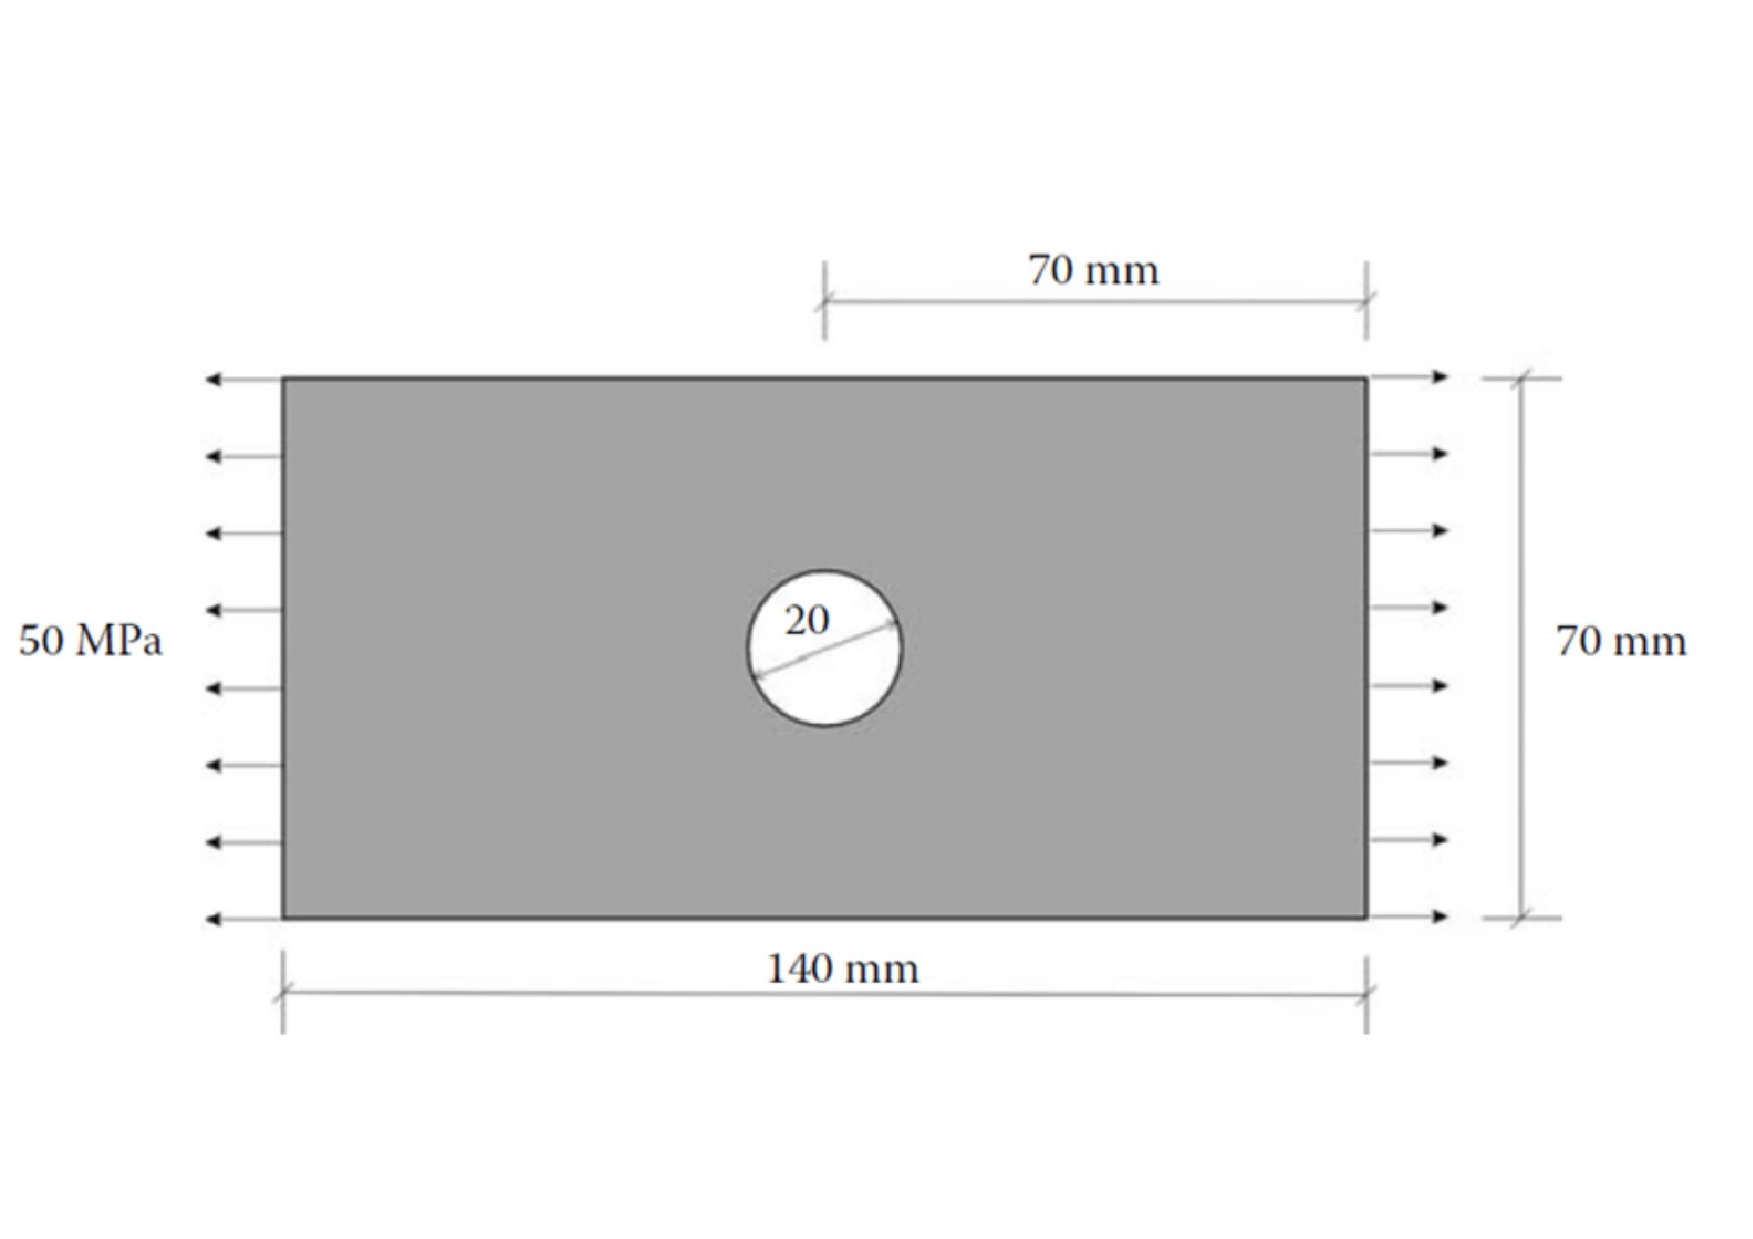
\includegraphics[width=0.70\textwidth]{figura}
\end{center}

\hrulefill
\vspace{4mm}

%%% end of the header

\shufflegroup{test1}
\insertgroup{test1}

\AMCcleardoublepage    
%\clearpage

\AMCformBegin    

%%% beginning of the answer sheet header

\noindent\AMCcode{nummat}{2}\hspace*{\fill}
\begin{minipage}{.7\linewidth}
$\longleftarrow{}$ Escriba su número de matrícula marcando los dígitos
en los recuadros (con ceros a la izquierda si el número es de menos de dos dígitos) y el nombre y apellidos debajo.

\vspace{3ex}

\namefield{\fbox{
   \begin{minipage}{.9\linewidth}
     Apellidos, Nombre:

     \vspace*{.5cm}\dotfill
     \vspace*{1mm}
   \end{minipage}
 }}
\end{minipage}

\begin{center}
 \bf\em Debe dar las respuestas exclusivamente en esta hoja (las respuestas en las demás hojas no serán tenidas en cuenta).
\end{center}

%%% end of the answer sheet header


\AMCform    

\AMCcleardoublepage    

}  

\end{document}
